Statistics Denmark (Danmarks Statistik) published a population projection in 2018 indicating that population growth in Denmark is primarily driven by an increase in the elderly population. According to the projection, the number of individuals aged over 80 is expected to increase to 2.5 times the 2018 level by 2057. This implies that, from 2053 onwards, it is projected that every tenth citizen will be over the age of 80\cite{noauthor_nyt_nodate}. The interest organization Ældre Sagen published an article in 2023 stating that the demographic group aged 65 and above accounts for one fifth of the population in Denmark \cite{noauthor_aeldre_nodate}.

\begin{figure}[H]
    \centering
    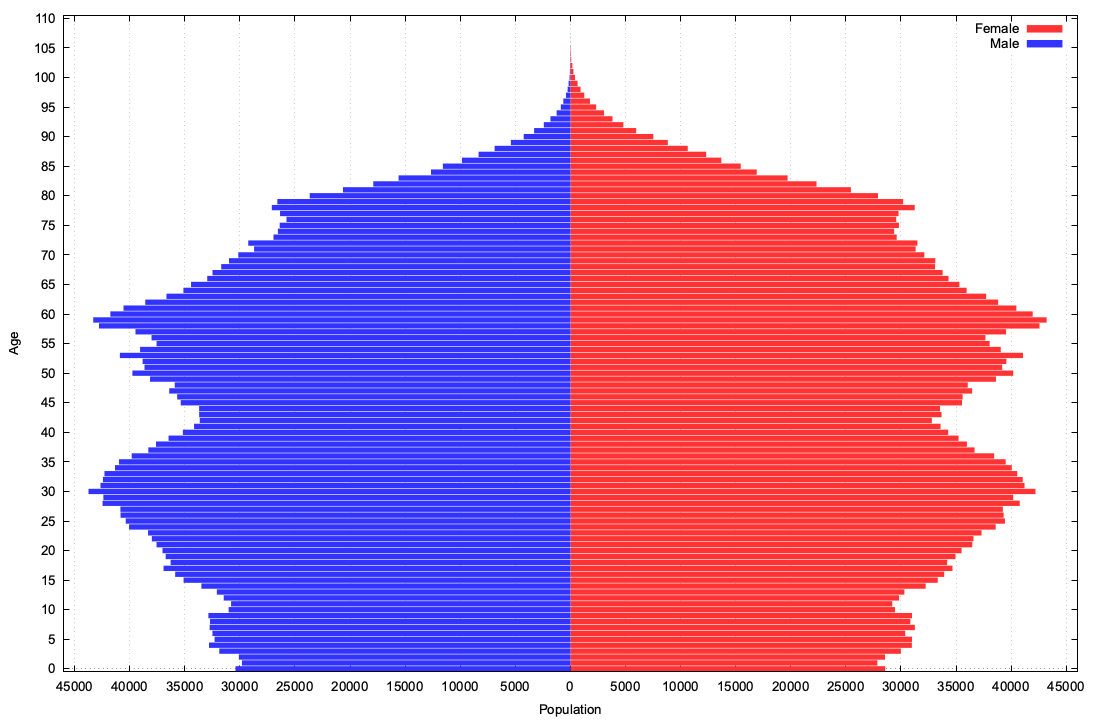
\includegraphics[width=\textwidth]{report/images/pop_pyramid_2025.png}
    \caption{People population pyramid for Denmark September 2025 made with data from \cite{noauthor_befolkningen_nodate}.}
    \label{fig:pop2025}
\end{figure}

\autoref{fig:pop2025} and \autoref{fig:pop2070} shows the population pyramids for 2025 and 2070, build on data from Statistics Denmark \cite{noauthor_befolkningen_nodate}. A population pyramid is a graphical representation of the age and gender distribution of a population. As shown in \autoref{fig:pop2025}, the demographic remains approximately the same in size up to the age of 60, after which a decline in the population is observed. In contrast, \autoref{fig:pop2070}, which provides a visual representation of the population projection for the year 2070, shows that the demographic maintains a similar size up to the age of 75, after which it begins to decrease. This reflects an increase in life expectancy. Furthermore, the population projection shown in \autoref{fig:pop2070} indicates that the number of individuals aged 0 to 20 is smaller than the number of individuals aged 20 to 75. This serves as an additional indicator that, at some point, there will be fewer people available to care for the elderly population.

\begin{figure}[H]
    \centering
    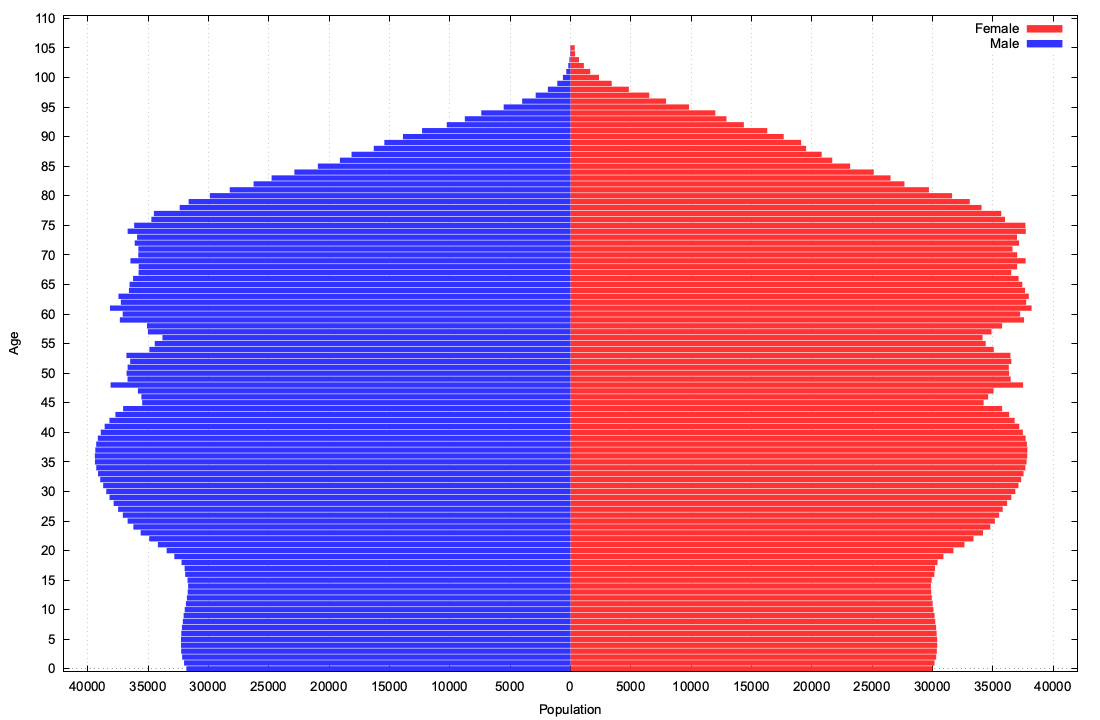
\includegraphics[width=\textwidth]{report/images/pop_pyramid_2070.png}
    \caption{Population pyramid for Denmark 2070 made with data from \cite{noauthor_befolkningsfremskrivning_nodate}.}
    \label{fig:pop2070}
\end{figure}


Danish Regions (Danske Regioner), an interest organisation for the five regions in Denmark, made calculations on the health expenditures of people based on their age. This data, which was found based on the Danish national patient registry and Statistics Denmark, found that the average health expenditure of a 66-70-year-old in 2021 was 23.000 DKK, while the average health expenditure for an 81-85-year-old was 36.000 DKK,\cite{noauthor_faktaark_flereaelre-uhi2pdf_nodate} as seen in the graph below (see \autoref{fig:elderly_expenditure}).

\begin{figure}[H]
    \centering
    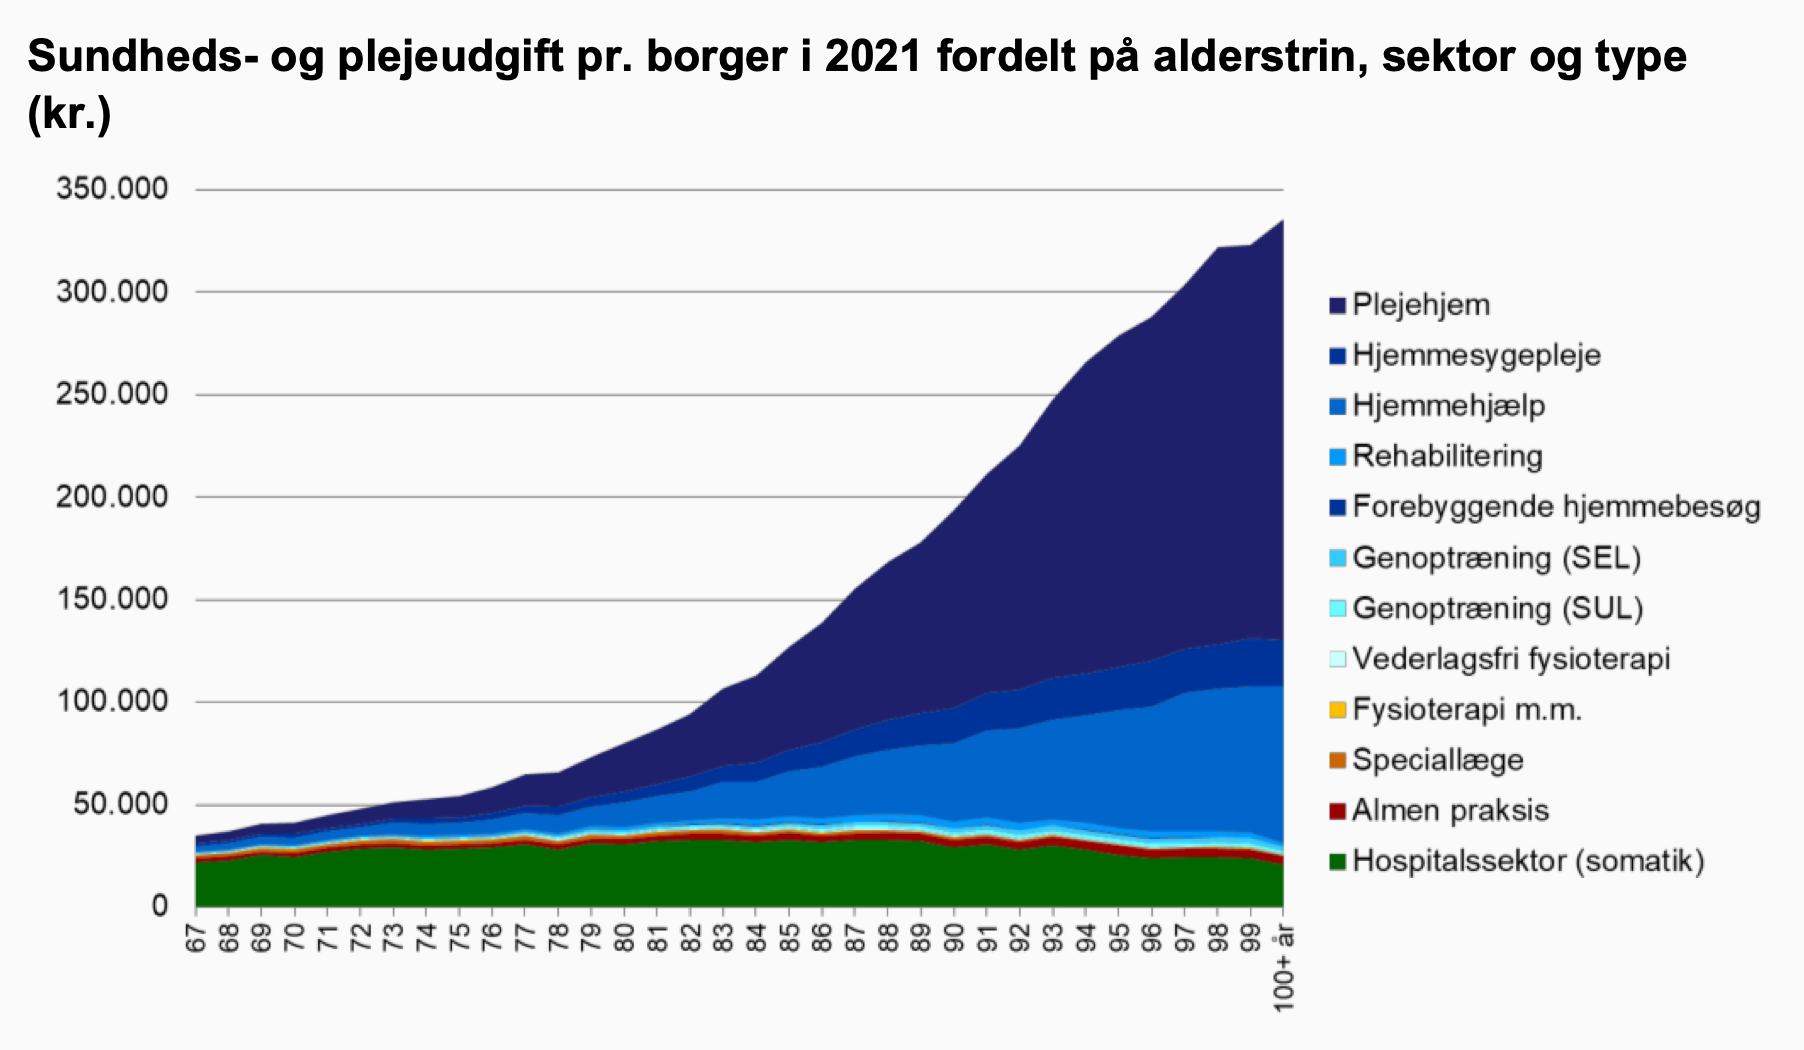
\includegraphics[width=\linewidth]{report/images/expenses-elders.png}
    \caption{Expenditure of citizens in Denmark by age group (in DKK)~\cite{kleist_aldersfordelte_2023}}
    \label{fig:elderly_expenditure}
\end{figure}

 The Danish patient handbook (Patienthåndbogen) states that about 33\% of people over the age of 65 fall at least once a year, and that 50\% of those people will fall more than twice a year \cite{noauthor_fald_nodate}. According to the Danish Health Authority (Sundhedsstyrrelsen), the most common injury for elderly people is falling \cite{noauthor_forebyggelse_nodate}. Furthermore, the Danish Health Authority found that the elderly population is two to three times more likely to fall, if you have fallen once in the span of a year. This however is only if no action is taken to prevent a similar fall from happening again. 